\chapter{Retrospective analyzer system}

This chapter is focused on the complementary software that has been added to this master thesis. Building on the approaches introduced \autoref{ch:retroDedGams} and the ones that were actually implemented in Intel Technology Poland presented in the chapter \autoref{ch:gamesDepl}, we created a web service, which helps scrum masters to choose a game suitable for the team.
The Retrospective analyzer system was created especially for Scrum Masters, Team Leaders and Managers in order to help them find a suitable game for the retrospective meeting. Leading a team is a difficult assignment, but thanks to Scrum, this job is being simplified. In order to make it more easy, we created a system that chooses a retrospective game for the team. What is more, we created a base of verified games with descriptions, in order to present a user with the different retrospective techniques our system provides. 

\section{System overview}

The Retrospective analyzer application is a web service. On \autoref{fig:welcomePage}, the welcome page is presented with an introduction what the system is offering.

\begin{figure}[h]
\caption{Welcome page screenshot}
\label{fig:welcomePage}
\centering
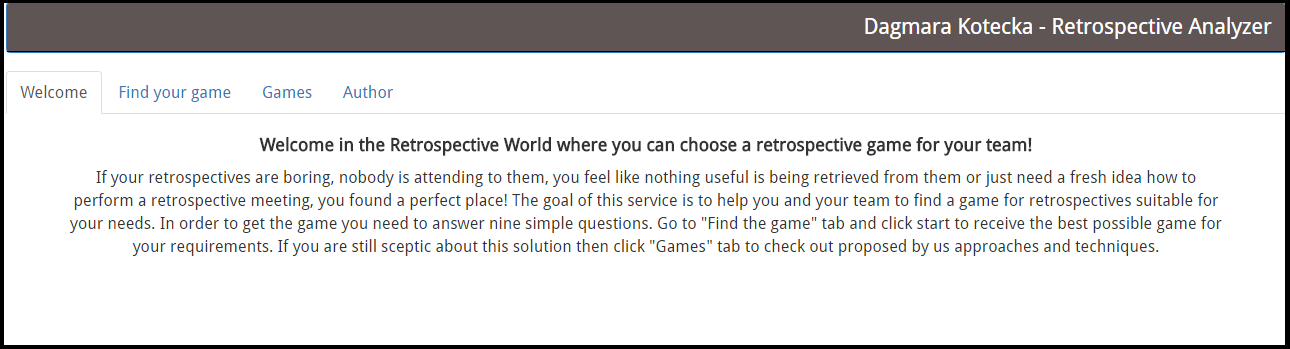
\includegraphics[width=1\textwidth]{screenshots/welcome.png}
\end{figure}

The Games tab is presented on the \autoref{fig:gamesPage} and it contains all the games included in this system.

\begin{figure}[h]
\caption{Games page screenshot}
\label{fig:gamesPage}
\centering
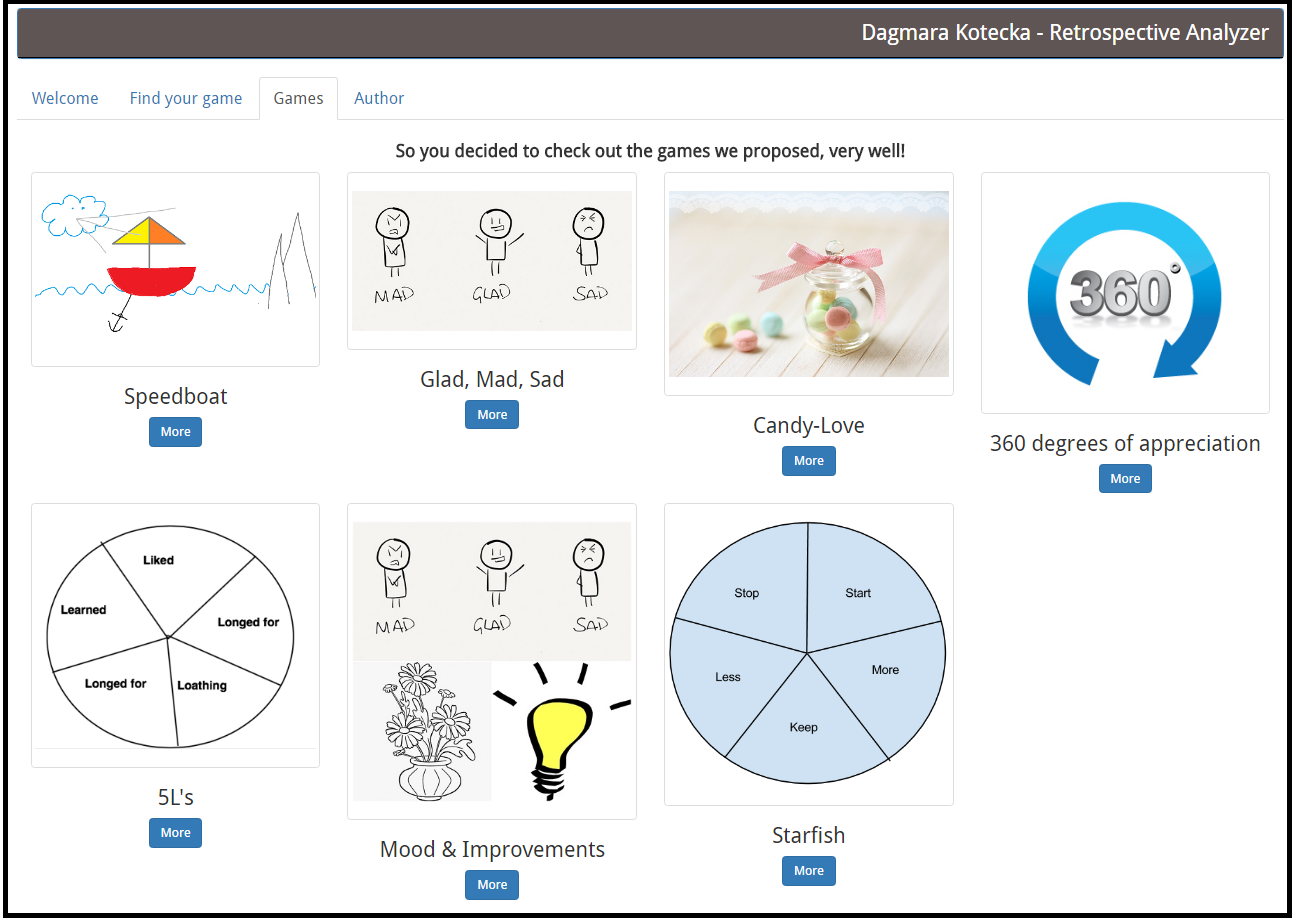
\includegraphics[width=1\textwidth]{screenshots/games.png}
\end{figure}

Another subpage and the most important one is the "Find The Game" tab, where the main functionality of the system is introduced. From this subpage, after clicking the start button shown on \autoref{fig:findGame}, the user is redirected to the page with questions presented on \autoref{fig:questionsPage}. The question page corresponds to the main issues which may occur in the Scrum team. Based on users answers, the system chooses the most suitable retrospective approach.

\begin{figure}[h]
\caption{Find game screenshot}
\label{fig:findGame}
\centering
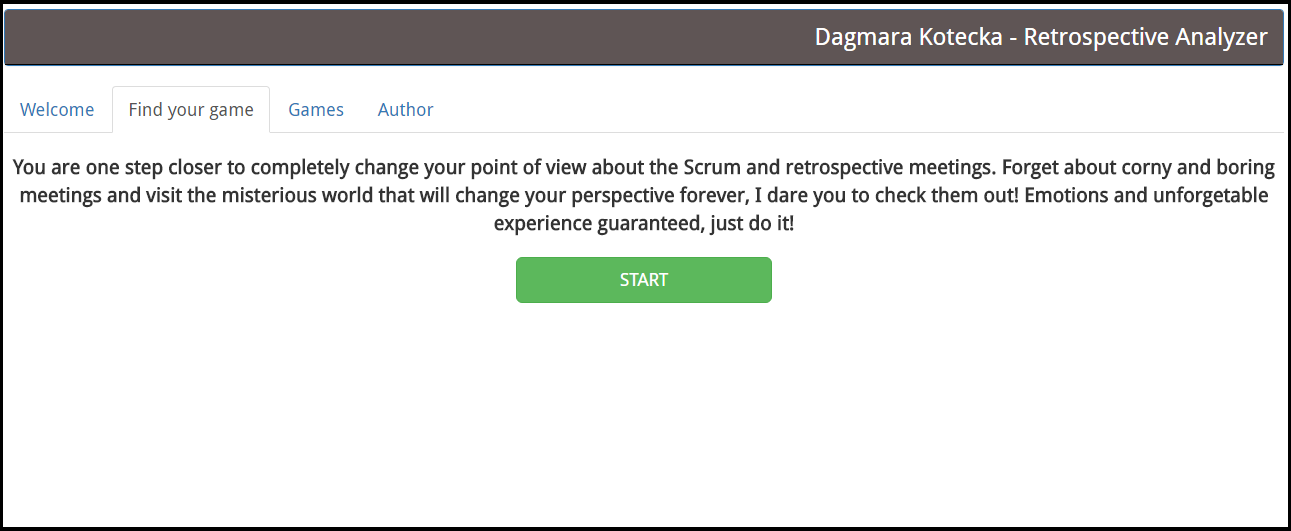
\includegraphics[width=1\textwidth]{screenshots/find.png}
\end{figure}

\begin{figure}[h]
\caption{Questions page screenshot}
\label{fig:questionsPage}
\centering
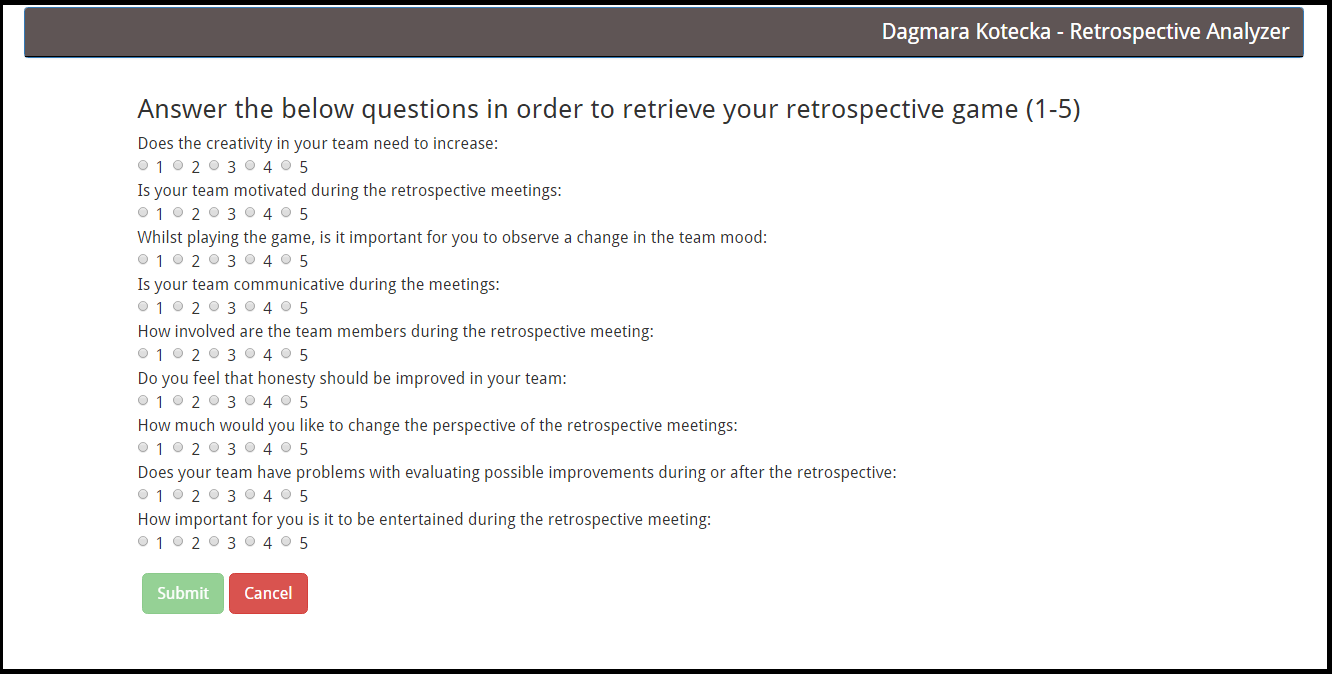
\includegraphics[width=1\textwidth]{screenshots/questions.png}
\end{figure}

The questions in the set were created based on \autoref{fig:gamesPoints}, which shows how many points the game reached in a particular factor using a scale from 1 to 10, where 1 is the lowest value and 10 the highest. The table has been created in association with Grzegorz Reglinski, the Intel Technology Scrum Master. We evaluated the table using feedback from the teams, our scrum experience and on the data collected from the survey.

Overall, "360-degrees of appreciation" was granted the highest sum whereas "Glad, Mad, Sad" received the lowest amount. The rest of the games' summary points fluctuates around a value of 50.

The chosen factors included in the table presented on \autoref{fig:gamesPoints} are as follows:
\begin{enumerate}
    \item Creativity - how the game influences the creativity of the team members.
    \item Team mood - this factor is useful for the team leaders and managers and thanks to this, they are able to notice what team mood is and react accordingly.
    \item Collaboration - this characteristic refers to how the game affects the cooperation of the team members while performing the retrospective meeting. 
    \item Communication - this element indicates whether the proposed approach enhances the discussions during the meeting.
    \item Degree of involvement - shows whether the proposed game increases the involvement of the participants.
    \item Change of perspective - indicates how different the approach is compared to the standard procedures and how big an impact the proposed game imposes on the change of the perspective.
    \item Honesty - this indicates whether we can observe an increase in honesty amongst the participants whilst they are playing the game.
    \item Entertainment - this factor presents how much amusement the game brought to the retrospective meeting.
    \item Improvement - indicates how much the game supports the team in terms of proposing ideas for improvements.
\end{enumerate}

Moreover, the nine factors above indicates which game will be retrieved after answering a set questions using a scale 1-5, where 1 is the user strongly disagrees and 5 is strongly agree. The nine questions are listed as follows (also listed on \autoref{fig:questionsPage}):
\begin{enumerate}
    \item Does the creativity in your team need to increase? 
    \item Is your team motivated during the retrospective meetings? 
    \item Whilst playing the game, is it important for you to observe a change in the team mood? 
    \item Is your team communicative during the meetings?
    \item How involved are the team members during the retrospective meeting?
    \item Do you feel that honesty should be improved in your team?
    \item How much would you like to change the perspective of the retrospective meetings?
    \item Does your team have problems with evaluating possible improvements during or after the retrospective?
    \item How important for you is it to be entertained during the retrospective meeting?
\end{enumerate}

The implemented algorithm of choosing the game is written in JavaScript and is presented below in \autoref{lst:jsAlg}:

\begin{lstlisting}[float=ht,escapechar=@,
    language=JavaScript,
    caption={The algorithm of choosing the game in JavaScript},
    label={lst:jsAlg},
    basicstyle=\ttfamily,
    keywordstyle=\color{blue}\ttfamily,
    stringstyle=\color{red}\ttfamily,
    captionpos=b,
    aboveskip=20pt,
    frame=trbl]

while (arr.indexOf("1") !== -1 || arr.indexOf("2") !== -1 ||
        arr.indexOf("3") !== -1 || arr.indexOf("4") !== -1 || 
        arr.indexOf("5") !== -1) {
        getMaxIndexes(arr, function () {
            changeMaxToZero(function () {
                getGames(function () {
                    reduceGames();
                });
            });
        })
    }
    
\end{lstlisting}

The server receives the data and parses it into the temporary array, \textit{arr}. Afterwards, it is passed into the while loop which is continuously executed until the array stops containing values between 1-5. The first function, \textit{getMaxIndexes} returns indexes of elements from the array that currently have a maxiumum value. The \textit{changeMaxToZero} procedure sets the values of the returned elements from  \textit{getMaxIndexes} to 0. Upon retrieving taking these indexes, the latter is mapped to the factors defined in \autoref{fig:gamesPoints} in the \textit{getGames} function and the ones with a
\[factorsValue >= (MAX * 2) - 1\]
are saved and stored in a global \textit{tmpArray} along with the \textit{max} value which ultimately determines the weight of the game. If the \textit{returnGames} array is empty then the \textit{reduceGames} function assigns the \textit{tmpArray} to the \textit{returnGames}. When the \textit{returnGames} array is not empty, it makes a sum of the \textit{max} with the already stored in it value
\[value[i] = value[i] + max  \].

If the array does not contain values of 1-,5 the game with the highest weight is being returned and:
\begin{enumerate}
    \item If the \textit{returnGames} array has more than 1 element, then the all of the games are viewed to the user.
    \item If the \textit{returnGames} array contains 1 element, the game is shown to the user.
\end{enumerate}

The source of this system has been open-sourced and can be found under this link \url{https://github.com/dagkotecka/Retrospective-Analyzer}.

\begin{figure}[h]
\caption{Games points table}
\label{fig:gamesPoints}
\centering
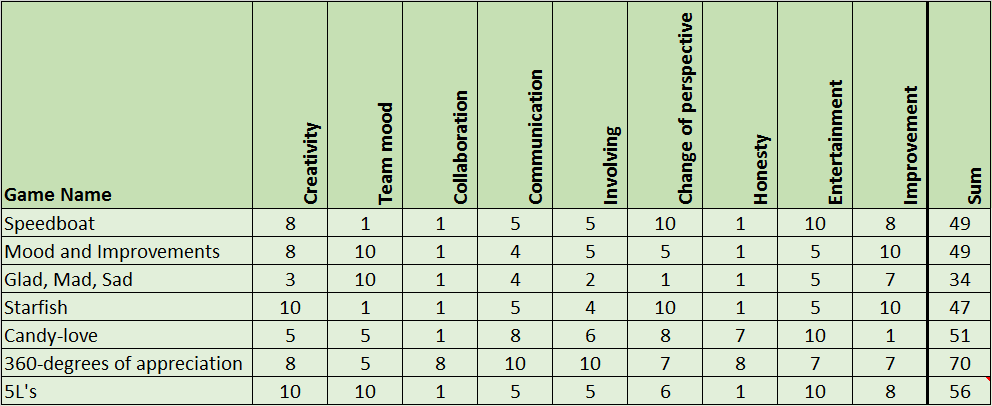
\includegraphics[width=1\textwidth]{screenshots/gamesPoints.png}
\end{figure}

After the user answers the questions, the system returns the game and a reference (as a button) to its description. This page is presented on the \autoref{fig:retrievedGame}.

\begin{figure}[h]
\caption{Retrieved Game page screenshot}
\label{fig:retrievedGame}
\centering
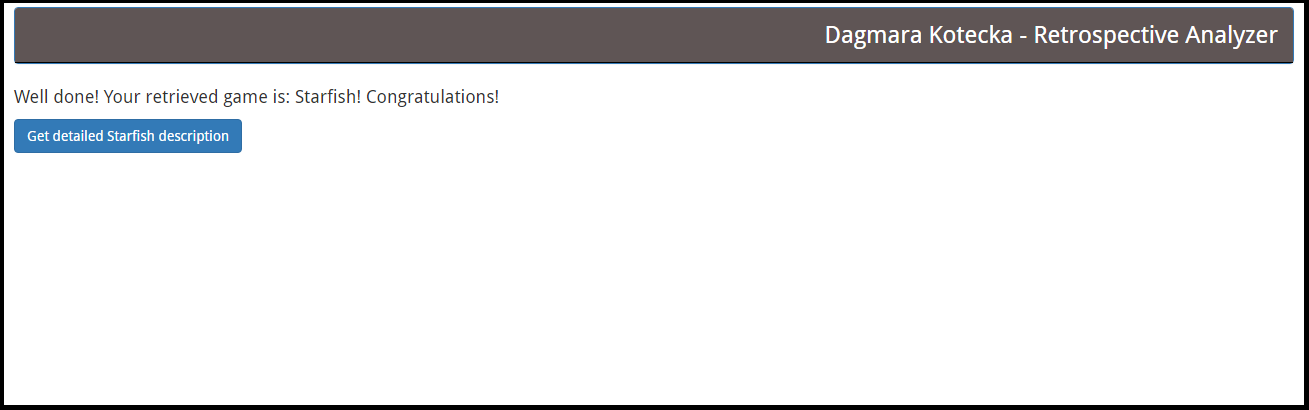
\includegraphics[width=1\textwidth]{screenshots/retrievedGame.png}
\end{figure}

There are two ways of accessing the game description page shown on \autoref{fig:gameDescPage}. The first way is to access it via the Games Page (\autoref{fig:gamesPage}). The second way, after filling the form on the questions page and retrieving the game from the system, is to click the description button on the Retrieve Game page (\autoref{fig:retrievedGame}). The game description contains the game name, the rules and the expected goal after playing the game. 

\begin{figure}[h]
\caption{Game description page screenshot}
\label{fig:gameDescPage}
\centering
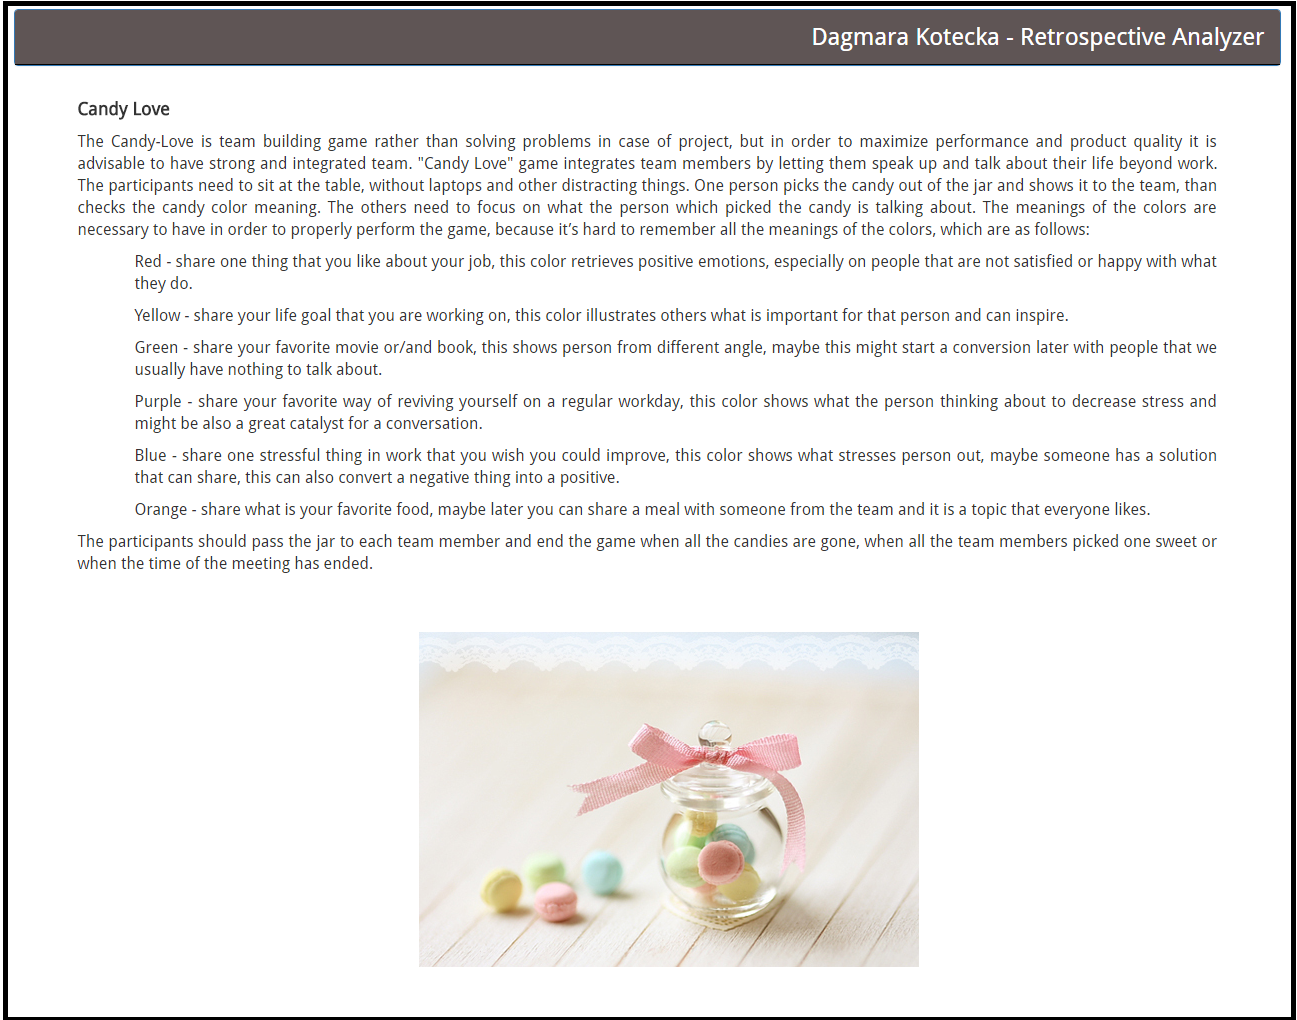
\includegraphics[width=1\textwidth]{screenshots/gameDesc.png}
\end{figure}

The use cases of the software are presented on \autoref{fig:useCases}. The retrospective meetings are led by developers which include the Scum Master, manager, team leaders and the developers. There are two use cases, where the first one is about viewing games and the second is about answering questions.

Both the backend and frontend of the software has been written using Visual Studio 2015 with a NodeJS extension on the Windows 8.1 platform. The tests have been executed on Google Chrome version 51, Internet Explorer version 11 and Mozilla Firefox version 37 browsers. The results of the evaluation were successful.

\begin{figure}[h]
\caption{System use cases}
\label{fig:useCases}
\centering
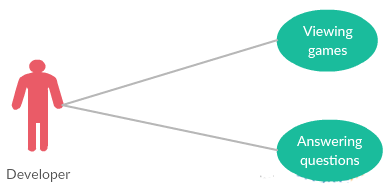
\includegraphics[width=0.5\textwidth]{img/useCases}
\end{figure}

\section{Backend architecture}

The backend is written in the NodeJS, which is an asynchronous event driven by JavaScript runtime and it has been designed in order to build scalable network applications. The Google's V8 JavaScript engine interprets JavaScript in the runtime environment. NodeJS enables the creation of servers without using threading and it uses the model of event-driven programming that uses callbacks in order to signal the completion of the task.

The backend framework was chosen from the a variety of available possibilities for a number of reasons. Firstly, both the backend and the frontend can be written in JavaScript, which means there is no switching between languages and also, this means the build process can be simplified. What is more, NodeJS is distinctly faster than for example Java or PHP, as there are no threads and no overheads that slow down the service.

The data is stored in Random Access Memory (RAM), because there is no need to keep it in any database. The game descriptions are rendered by being redirecting to the endpoint with the game name and the table presented on \autoref{fig:gamesPoints}. The factors are stored in a JSON object, which is a natural part and the foundation of JavaScript and can be used without including any libraries. The other reason to not detain the data in the database is the time-consuming communication between the system and the storage. Moreover, the data was so small that it would have been pointless to store it in a database. 

\autoref{tab:viewingRest} shows the API Rest calls made to the NodeJS server. The first call was made in order to retrieve the game from the server, using the listed factors in \autoref{fig:gamesPoints} factors as parameters. The second call as listed in \autoref{tab:viewingRest} is to render the page with the game description. This does not take any parameters.

\begin{table}[h]
	\caption{Rest API calls}
	\label{tab:viewingRest}
	\begin{tabularx}{\textwidth}{|X|X|X|X|X|}
	\hline
		Type of HTTP Request & URL & Parameters & On Success & Description \\ \hline
		/POST &  /{gameName} & creativity, collaboration, teammood, communication, involvement, honesty, perspective, improvement, entertainment & Returns a game & Call  to  server  to retrieve the game after answering  on a set of questions \\ \hline
		/GET & /getGame & None & Renders Page & Rendering a description page of the games. \\ \hline
	\end{tabularx}
\end{table}

For the purpose of maintaining the pages Express has been used, which is minimal and flexible NodeJS web application framework. Thanks to Express, it is easy to create a server using just a few lines. The declaration of endpoints and REST Api calls is very simple and compared to the main competitors of the Express framework, the Koa and the Hapi, it has the biggest community and is the most mature and reliable framework. What is more, it promotes code reusal with its built in router.

\section{Frontend structure}

While implementing the frontend of the retrospective, the main goal was to create a simple, intuitive and responsive design. In order to simplify the interface, a bootstrap framework has been used. Thanks to the bootstrap framework, the website is able to scale and is properly viewed on phones, tablets and desktops with the CSS media queries.

The choice for the framework that would ease and allow developers to create a responsive design of the responsive website has been made between two of the most popular and well documented solutions. The retrieved candidates were Bootstrap and Foundation. The main reason why the Bootstrap framework has been chosen, was that we have already implemented services using the framework and also, we have experience in that field. The comparison presented in \autoref{tab:compBootFound} shows that both frameworks have very similar specifications and without the advantage of our experience in Bootstrap, it would not make difference in terms of choosing which framework to use. The main advantages of Bootstrap are the support for all the modern browsers and the bigger community support. What is more, the code is clean and readable when using the Bootstrap framework. Moreover, it is easy to find the examples and tutorials on how to implement a particular element. The components of the Bootstrap are well documented.

\begin{table}[ht!]
\caption{A comparison between Bootstrap and Foundation}
\label{tab:compBootFound}
\begin{tabularx}{\textwidth}{|X|X|X|}
\hline
\textbf{Comparison area} & \textbf{Bootstrap} & \textbf{Foundation}  \\ \hline
Browser support & all modern web browsers & lack of Internet Explorer 8 support \\ \hline
Community support & bigger than Foundation & smaller than Bootstrap \\ \hline
Performance & similar to Foundation & similar to Bootstrap \\ \hline
Layout definition & easy & easier \\ \hline
Sizing units & pixels & rems (equals to the font size of root element)\\ \hline
Form validation & not so easy at the beginning & effortless (\textit{Abide}) \\ \hline
\end{tabularx}
\end{table}

Even though HTML has been a foundation of the web we decided to make use of a more modern approach. Accordingly, Jade was designed at the beginning for server-side templating in NodeJS, but in our solution it has been used as a short hand for HTML. Using Jade has made the code cleaner and there was no need to use ending tags. Jade uses whitespaces and indentation as part of its language, so in order to properly render a page, it is crucial that you are careful and follow the proper syntax. What is more, Jade offers an easy way to write conditions and iterators, which as a result, gives rise to shorter codes. An example is presented on \autoref{fig:jadeHtml}.

\begin{figure}[ht!]
\caption{The same layout defined in Jade and HTML}
\label{fig:jadeHtml}
\centering
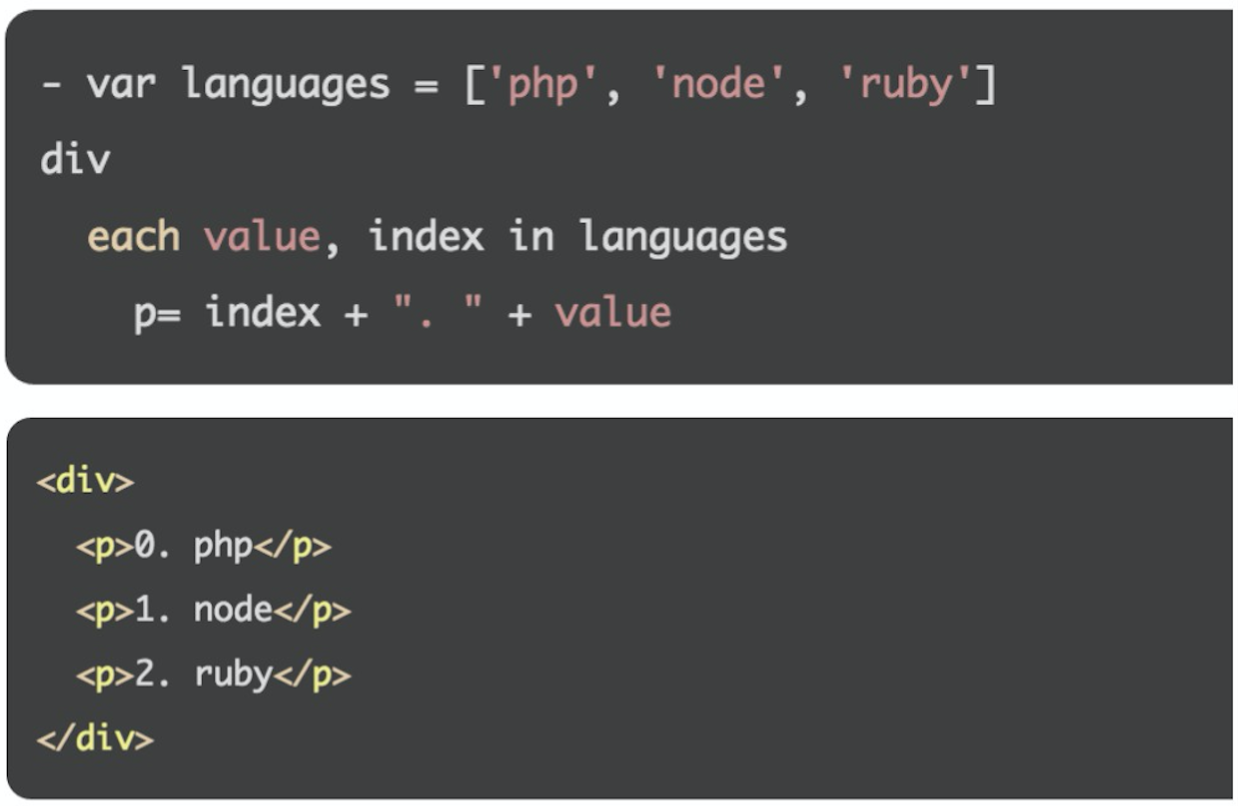
\includegraphics[width=0.5\textwidth]{img/htmlJade}
\end{figure}

\section{System evaluation}

The web service evaluation has been made in Intel Technology Poland in Gdansk. The Scrum Master, Grzegorz Reglinski, after testing the software, has made a few suggestions. In our company, the Retrospective has been the least appreciated meeting in Scrum and the task of encouraging team members to actively participate is a difficult job. Grzegorz thinks that the Retrospective Analyzer is very useful in terms of supporting the leader, who performs the activity. He found the software is very easy to use, the interface is intuitive, the layout is simple and it does not contain any useless content. What is more, he tested the main functionality of the web-service and the game retrieval, and as a result was satisfied with the outcome. The answers on the input questions suited the game he wanted to get. He also noticed that the retrospective approaches are easy to understand and have an interesting description. Grzegorz found the pictures and the description very important in order to properly perform the game. He suggested a few improvements and two out three of them have been added to the software: 
\begin{enumerate}
    \item The welcome page should contain a picture of the flow and how the game retrieval functionality works. This is because pictures tend to express more than words. The suggested improvement is presented on \autoref{fig:welcomePageImpr}.
    \item The questions should have bigger spaces between each other and instead of a number describing the opinion, a statement should be used. For example, instead of 5, there could be "the team is very creative, has plenty of ideas and is eager to share them". The suggested improvement was added to the backlog.
    \item Each game description should contain the evaluated points presented in \autoref{fig:gamesPoints}. The suggested improvement is presented on \autoref{fig:gamePageImpr}.
\end{enumerate}

\begin{figure}[ht!]
\caption{The improved Welcome Page}
\label{fig:welcomePageImpr}
\centering
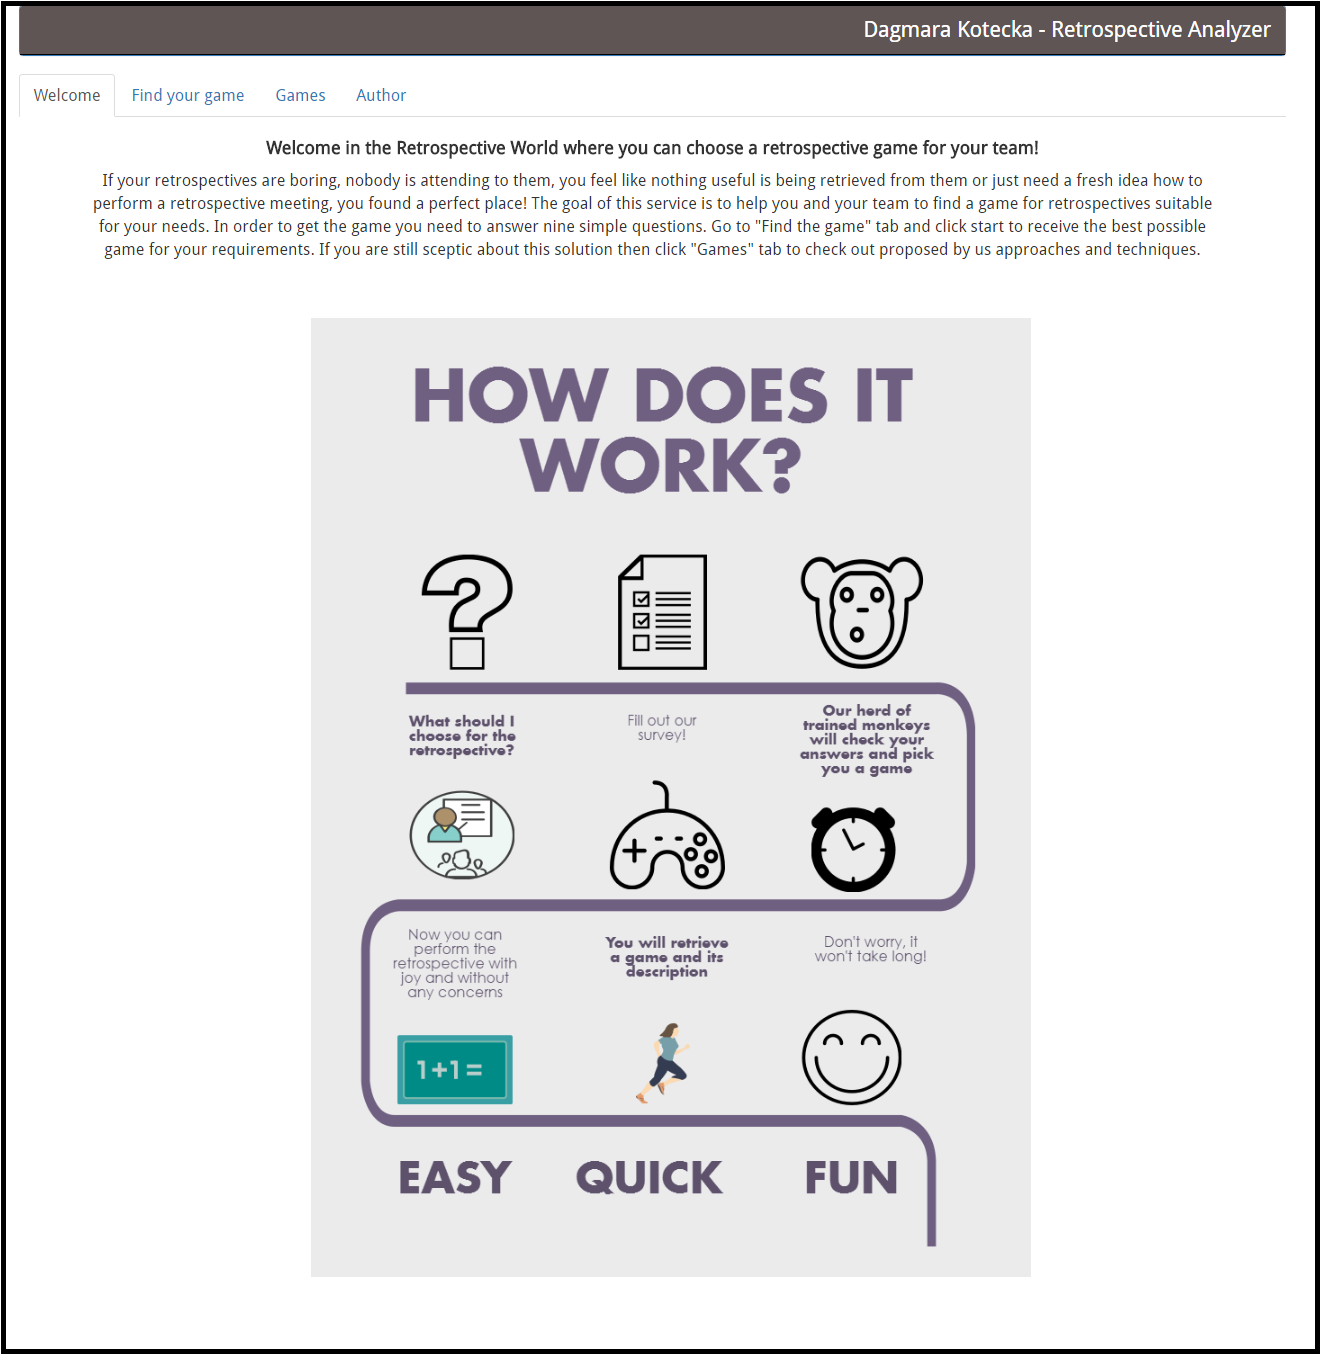
\includegraphics[width=1.0\textwidth]{img/newWelcome}
\end{figure}

\begin{figure}[ht!]
\caption{The improved Game Page with the Game Points included}
\label{fig:gamePageImpr}
\centering
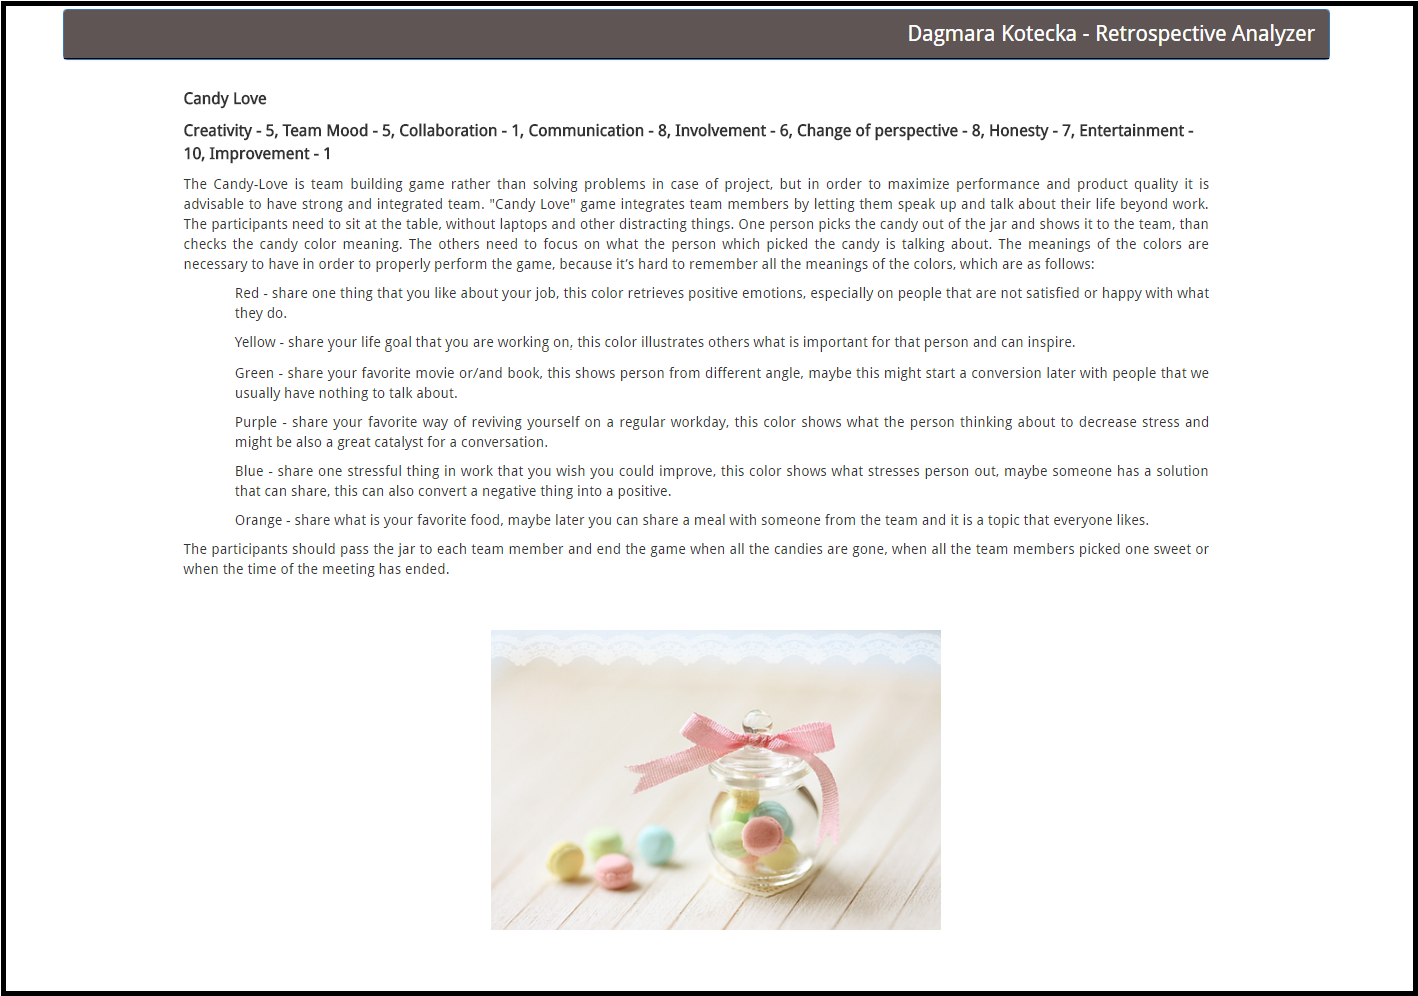
\includegraphics[width=1.0\textwidth]{img/newGame}
\end{figure}

What is more, this complementary Retrospective Analyzer web service has implemented the "must have" features in order to show how many possibilities there are to help the developers to effectively perform the Scrum Retrospective meeting. There are plenty of planned features that would make the system more functional, but as it is with software,, the system must be completed within a given deadline. This is because the development of the service would last forever until someone would eventually say "Stop, that is enough". The possible features that might be included in the software in the future have been retrieved through valuable discussion with Grzegorz Reglinski and these are as follows:
\begin{enumerate}
    \item As a scrum master, I would like the system to allow the result to be affected by multiple users.
    \item As a scrum master, I would like to have the option to create separate groups for the team in order to maintain the results of each group.
    \item As a scrum master, I would like to have an admin panel where I can track the results of the game.
    \item As a user, I would like the questions to have bigger spaces between each other and instead of a number describing the opinion a statement. For example, instead of 5, there could be "the team is very creative, has plenty of ideas and is eager to share them".
\end{enumerate}



